\documentclass[12pt]{article}

\fontfamily{lmss}
\usepackage{fullpage}
\usepackage{amsmath}
\usepackage{amsthm}
\usepackage{url}
\usepackage{multicol}
\usepackage{enumerate}
\usepackage{graphicx}
\usepackage{color}
\usepackage{hyperref}
\hypersetup{
    colorlinks=true,
    linkcolor=blue,
    filecolor=magenta,      
    urlcolor=blue,
}

\usepackage{geometry}
\geometry{
  top=1in,            % <-- you want to adjust this
  bottom=1in,
  left=1in,
  right=1in,
  headheight=3ex,       % <-- and this
  headsep=4ex,          % <-- and this
}

\usepackage{lastpage}
\usepackage{fancyhdr}
\pagestyle{fancy}
\fancyhf{}
\renewcommand{\footrulewidth}{0.4pt}
\lhead{CS 486/686}
\rfoot{Page \thepage\ of \pageref{LastPage}}

\setlength{\parskip}{\baselineskip}%
\setlength{\parindent}{0pt}%

\usepackage{tcolorbox}
\tcbuselibrary{breakable}
\newenvironment{markscheme}
{
    \renewcommand{\parskip}{\baselineskip}
    \begin{tcolorbox}[
        colback=blue!10,
        colframe=blue!10,
        sharp corners,
        breakable
    ]
    \textbf{Marking Scheme:}
}
{
    \end{tcolorbox}
}

\newenvironment{sol}[1]{
\color{red}
	{\bf Solution:}
}{
}


\lfoot{\copyright Alice Gao 2021}
\chead{Winter 2021}
\rhead{Assignment 4}
\cfoot{v1.0}

\title{CS 486/686 Assignment 4 (76 marks)}
\author{Alice Gao}
\date{Due Date: 11:59 PM ET on Wednesday, April 14, 2021
with an extension with no penalty to 11:59 pm ET on Thursday, April 15, 2021}

\begin{document}

\maketitle

% \section*{Changes}

% \begin{itemize}
%     \item v1.1
% \end{itemize}
% \newpage

\newpage
\section*{Academic Integrity Statement}

I declare the following statements to be true:

\begin{itemize}
\item 
The work I submit here is entirely my own.

\item 	
I have not shared and will not share any of my code with anyone at any point. 

\item 
I have not posted and will not post my code on any public or private forum or website.

\item 	
I have not discussed and will not discuss the contents of this assessment with anyone at any point.

\item 
I have not posted and will not post the contents of this assessment and its solutions on any public or private forum or website. 

\item 
I will not search for assessment solutions online.

\item 
I am aware that misconduct related to assessments can result in significant penalties, possibly including failure in the course and suspension. This is covered in Policy 71: https://uwaterloo.ca/secretariat/policies-procedures-guidelines/policy-71.
\end{itemize}

Failure to accept the integrity policy will result in your assignment not being graded.

By typing or writing my full legal name below, I confirm that I have read and understood the academic integrity statement above.



\newpage
\section*{Instructions}

\begin{itemize}
\item
Submit the assignment in the A4 Dropbox on Learn. 
No late assignment will be accepted. This assignment is to be done individually.

\item 
I strongly encourage you to complete your write-up in Latex, using this source file. If you do, in your submission, please replace the author with your name and student number. Please also remove the due date, the Instructions section, and the Learning goals section. 
\item
Lead TAs: 
\begin{itemize}
\item
Ethan Ward (\href{mailto:e7ward@uwaterloo.ca}{e7ward@uwaterloo.ca})
\end{itemize}
The TAs' office hours will be posted on MS Teams.
\item
Submit two files with the following names.

\begin{itemize}
\item
{\bf writeup.pdf}

\begin{itemize}
\item
Include your name, email address and student ID in the writeup file.
\item
If you hand-write your solutions, make sure your handwriting is legible and take good quality pictures. You may get a mark of 0 if we cannot read your handwriting.

\end{itemize}
\item
{\bf code.zip}

\begin{itemize}
\item
This zip file includes any other relevant files for your submission.

\end{itemize}

\end{itemize}
\end{itemize}



\section*{Learning goals}

{\bf Decision Networks}

\begin{itemize}
\item 
Model a real-world problem as a decision network with sequential decisions.
\item
Given a decision network with sequential decisions, determine the optimal policy and the expected utility of the optimal policy by applying the variable elimination algorithm.
\end{itemize}

{\bf Markov Decision Process}
\begin{itemize}
\item
Trace the execution of and implement the value iteration algorithm to solve a Markov decision process.
\end{itemize}


\newpage
\section{Decision Network for ``Monty Hall'' (28 marks)}

The Monty Hall Problem is stated as follows.

You are on a game show, and you are given the choice of three doors: Behind one door is a car; behind the others, goats. The host knows what's behind each door but you don't.

\begin{itemize}

\item 
First, you pick a door, say Door 1.

\item 
Second, the host opens another door, say Door 3, which has a goat behind it.

\item 
Finally, the host says to you, ``Do you want to pick Door 2?'' 
\end{itemize}

Is it to your advantage to switch your choice? 

The host always opens a door with a goat behind it, but not the door you chose first, regardless of which door you chose first. You ``reserve'' the right to open the door you chose first, but can change to the remaining door after the host opens the door to reveal a goat. You get as a price the item behind the final door you choose. You prefer cars over goats (cars are worth 1 and goats are worth 0). The car is behind doors 1, 2, and 3 with probabilities $p_1$, $p_2$ and $1 - p_1 - p_2$ respectively, and you know the values of $p_1$ and $p_2$.

Model this problem using a decision network using the following variables.
    
\begin{itemize}

\item CarDoor $\in \{ 1, 2, 3\}$ is the door such that the car is behind it. This is a random variable.

\item FirstChoice $\in \{1, 2, 3\}$ is the index of the door you picked first. This is a decision variable.

\item HostChoice $\in \{smaller, bigger\}$ is the index of the door picked by the host. The value of this variable indicates whether the index of the door picked is the smaller or bigger one of the two doors left after you made your first choice. This is a random variable.
    
\item SecondChoice $\in \{stay, switch\}$ indicates whether you stay with the door you picked first or switch to the remaining door not opened by the host. This is a decision variable.

\item Utility $\in \{0, 1\}$ is 0 if you get a goat and 1 if you get a car. 

\end{itemize}


Please complete the following tasks.

\begin{enumerate}

\item     
Complete the decision network in Figure~\ref{fig:monty_hall} by drawing all the arcs. Show the probability table for each random variable. Show the utility table for the utility node. You can use $p_1$ and $p_2$ in your tables since you do not know their values yet.

Hint: When you are deciding whether node A should be a parent of node B (a decision variable), think of the following. If node A is a parent of node B, then the optimal policy may be of a form that: if A has value a, then B should be b. Otherwise, if node A is not a parent of node B, the optimal policy for B cannot depend on the value of A. In other worlds, adding an edge in the network increases the set of possible policies that we would consider. 
    
\begin{figure}[ht!]
\centering
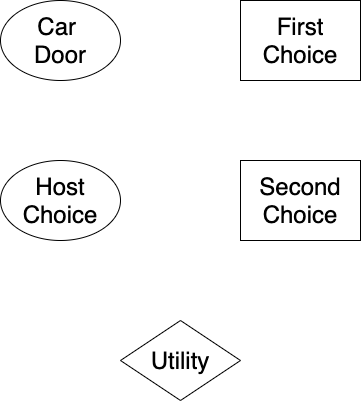
\includegraphics[width=0.4\textwidth]{images_posted/a4-dn1-empty.png}
\caption{The Monty Hall Problem}
\label{fig:monty_hall}
\end{figure}
    
\begin{markscheme}

(10 marks)

\begin{itemize}
    \item (4 marks) Correct parent nodes.
    \item (3 marks) Correct probability tables.
    \item (3 marks) Correct utility table.
\end{itemize}

\end{markscheme}


\item

{\bf Assume that $p_1 = 1/3$ and $p_2 = 1/3$.}  

Compute the optimal policy for the decision network by applying the variable elimination algorithm. Show all your work including all the intermediate factors created. Clearly indicate the optimal policy and the expected utility of the agent following the optimal policy.

\begin{markscheme}

(9 marks)

\begin{itemize}
    \item (4 marks) Sum out variables in the correct order.
    \item (2 marks) Correct optimal policy for FirstChoice.
    \item (2 marks) Correct optimal policy for SecondChoice.
    \item (1 mark) Correct value of the expected utility of the optimal policy.
\end{itemize}    

\end{markscheme}
    
    
\item

Consider a different case where {\bf $p_1 = 0.7$ and $p_2 = 0.2$.}  The car is much more likely to be behind door 1 than to be behind door 2 or 3. The car is slightly more likely to be behind door 2 than to be behind door 3.

Compute the optimal policy for the decision network by using the variable elimination algorithm. Show all your work including all the intermediate factors created. Clearly indicate the optimal policy and the expected utility of the agent following the optimal policy.

\begin{markscheme}

(9 marks)

\begin{itemize}
\item (4 marks) Sum out variables in the correct order.
\item (2 marks) Correct optimal policy for FirstChoice.
\item (2 marks) Correct optimal policy for SecondChoice.
\item (1 mark) Correct value of the expected utility of the optimal policy.
\end{itemize}    

\end{markscheme}
    
      
\end{enumerate}






\newpage
\section{Reinforcement Learning (48 marks)}

You will explore two grid worlds similar to the one discussed in lecture by running the active version of the adaptive dynamic programming algorithm.

We will test your program on two grid worlds. See their descriptions in section~\ref{sec:worlds}.

Implement the {\bf adaptive dynamic programming} algorithm for {\bf active reinforcement learning}. Check section~\ref{sec:active_adp} for details and tips on implementing the active ADP algorithm.

{\bf What to submit:}

\begin{itemize}
\item In your \verb+writeup.pdf+, include the long-term utility values and the optimal policy for both worlds. 

\item In your \verb+code.zip+, include a bash script \verb+a4.sh+. When the TA runs \verb+bash a4.sh+, the script should run active ADP on both the \verb+lecture+ world and the \verb+a4+ world and print out the long-term utility values and the optimal policy for both worlds.
\end{itemize}

Please complete the following tasks.

\begin{enumerate}
\item For the \verb+lecture+ world, report the {\bf long-term utility values} for all the states learned by the active ADP algorithm. 

Because of randomness in the problem, your answers do not have to match our answers exactly. We will determine a range of acceptable values. As long as your values are within this range, you will get full marks.

\begin{markscheme}
(12 marks)

\begin{itemize}
    \item (6 marks) The TA can run your program to reproduce the long-term utility values within a minute.
    \item (6 marks) The reproduced long-term utility values are within the acceptable range.
\end{itemize}
\end{markscheme}


\item For the \verb+lecture+ world, report the {\bf optimal policy} given the long-term utility values. 

Similar to the previous part, we will mark your answers based on whether they match multiple possible answers.

\begin{markscheme}
(12 marks)

\begin{itemize}
    \item (6 marks) The TA can run your program to reproduce an optimal policy within a minute.
    \item (6 marks) The reproduced optimal policy matches a possible answer.
\end{itemize}
\end{markscheme}



\item For the \verb+a4+ grid world, report the {\bf long-term utility values} for all the states learned by the active ADP algorithm.

Similar to the previous parts, we will mark your answers based on whether they fall within the acceptable range of values.

\begin{markscheme}
(12 marks)

\begin{itemize}
    \item (6 marks) The TA can run your program to reproduce the long-term utility values within a minute.
    \item (6 marks) The reproduced long-term utility values are within the acceptable range.
\end{itemize}
\end{markscheme}




\item For the \verb+a4+ world, report the {\bf optimal policy} given the long-term utility values. 

Similar to the previous parts, we will mark your answers based on whether they match multiple possible answers.

\begin{markscheme}
(12 marks)

\begin{itemize}
    \item (6 marks) The TA can run your program to reproduce an optimal policy within a minute.
    \item (6 marks) The reproduced optimal policy matches a possible answer.
\end{itemize}
\end{markscheme}


\end{enumerate}

\subsection{The two grid worlds}
\label{sec:worlds}

We will test your program on two grid worlds. The \verb+lecture+ world is a version of the grid world discussed in lecture. The \verb+a4+ world is created for this assignment.

{\bf The \verb+lecture+ grid world}

The grid world discussed in lecture is given below. $S_{00}$ is the initial state. $S_{13}$ and $S_{23}$ are goal states. $S_{11}$ is a wall.
\begin{center}
\begin{tabular}{ | c | c | c | c | c |} \hline
& 0 & 1 & 2 & 3  \\ \hline
0& &     &  &  \\ \hline
1& & X &  & -1  \\ \hline
2& &     &  & +1 \\ \hline
\end{tabular}
\end{center}

For this world, you can assume the following.
\begin{itemize}
\item The immediate reward of entering any non-goal state is $-0.04$.
\item The transition probabilities:  The agent moves in the intended direction with probability $0.8$, moves to the left of the intended direction with probability $0.1$, and moves to the right of the intended direction with probability $0.1$.
\item 
The discount factor is 1.
\end{itemize}

{\bf The \verb+a4+ grid world}
\begin{itemize}
\item Each grid world has 4 columns and 3 rows.
\item Each world has at least one goal state. Entering any goal state causes the agent to exit the world.
\item The reward of entering a goal state is $1$ or $-1$.
% \item The maximum immediate reward of entering any state is $2$.
\item In a given world, there is a fixed immediate reward of entering any non-goal state. The immediate reward for entering every non-goal state is the same.
\item In each state, there are four available actions: up, down, left, and right. 
\item If the agent moves in a direction and hits a wall, the agent will stay in the same square.
\item By taking an action, it is possible for the agent to reach any of the four neighbouring squares (if there is a wall on any side, the neighbouring square is the current square the agent is in.).
\end{itemize}

The information for both grid worlds is provided through \verb+run_world.pyc+. The \verb+run_world.pyc+ was produced with {\bf Python 3.7.6}. The file includes the following functions. The \verb+world+ string can be \verb+lecture+ or \verb+a4+.

{\bf Do not decompile \verb+run_world.pyc+ and look at the code. That defeats the purpose of providing the pyc file. You should treat the grid world as a black box and build your program based on that.}

\begin{itemize}
\item \verb+get_gamma(world)+: Returns the discount factor given the world string. 

\item \verb+get_reward(world)+: Returns the immediate reward of entering any non-goal state given the world string. 

\item \verb+read_grid(world)+: Returns a numpy array representing the grid given the world string. 

In the grid, the meanings of the symbols are as follows.
\begin{itemize}
\item \verb+S+ is the initial state.
\item \verb+*+ is any other non-goal state.
\item \verb+X+ is a wall.
\item If the state is \verb+1+ or \verb+-1+, it is a goal state with the number as the reward of entering the goal state.
\end{itemize}

\item \verb+make_move(grid, curr_state, dir_intended, world)+:  Given the grid, the current state, the intended direction and the world string, make a move based on the transition probabilities and return the next state. 

A state is encoded as a tuple (i,j) where i is the row index ($0 \le i \le 2$) and j is the column index ($0 \le j \le 3$). 

The intended direction is 0 for up, 1 for right, 2 for down, and 3 for left.

\end{itemize}

In addition, \verb+run_world.pyc+ has a few other helper functions that you can use:

\begin{itemize}

\item \verb+get_next_states(grid, curr_state)+: Given a grid and the current state, return the next states for all actions. The returned array contains the next states for the actions up, right, down, and left, in this order. For example, the third element of the array is the next state if the agent ends up going down from the current state.

\item \verb+is_goal(grid, state)+: Returns true if the given state is a goal state and false otherwise. The \verb+grid+ parameter needs to be the one returned by \verb+read_grid+. This function checks whether the given state $(i,j)$ is \verb+1+ or \verb+-1+.

\item \verb+is_wall(grid, state)+: Returns true if the given state is a wall and false otherwise. The \verb+grid+ parameter needs to be the one returned by \verb+read_grid+. This function checks whether the given state $(i,j)$ is \verb+X+.

\item \verb+not_goal_and_wall(grid, state)+: Returns true if the given state is not a goal state and nor a wall.

\item \verb+pretty_print_policy(grid, policy)+: Prints a policy in a readable format where the actions are printed as up, right, down, and left. The \verb+grid+ parameter needs to be the one returned by \verb+read_grid+. 

The \verb+policy+ is a grid of the same shape except that each value is one of 0, 1, 2, 3 and represents an action (0 is up, 1 is right, 2 is down, and 3 is left.). To display the policy properly, make sure that you create the grid with \verb+dtype=np.int+ 

\end{itemize}


\subsection{Tips for implementing active ADP}
\label{sec:active_adp}

{\bf A high-level summary of the the active ADP algorithm is described below.}
\begin{itemize}
\item Learn the transition probabilities using the observed transitions.

\item Solve for the long-term utility values of the states iteratively by using the Bellman equations (given the immediate reward values and the estimated transition probabilities).

\item Solve for the optimal policy given the estimated long-term utility values of the states.

\item Move the agent and determine the next state based on the optimal policy for the current state.

\item Repeat the steps above until the long-term utility values converge.
\end{itemize}

Your active ADP algorithm should keep track of the following information. 
\begin{itemize}

\item $N(s,a)$: the number of times that we have visited a given state-action pair.

\item $N(s,a,s')$: the number of times we have reached state $s'$ by taking action $a$ in state $s$.

\item $V(s)$: The long-term expected utility of state $s$. Use a 2D numpy array to store the long-term utility value for each state in the grid world.


\end{itemize}

{\bf A detailed description of the active ADP algorithm is given below.}
\begin{enumerate}

\item Given the grid, the current utility estimates, the current state, and the counts $N(s,a)$ and $N(s,a,s')$, determine the best action as follows.
    
\begin{align}
& \arg\max_a f \left( \sum_{s'} P(s'|s,a) V(s'), N(s,a) \right) \\
& f(u,n) = 
\begin{cases}
R^+, \text{ if } n < N_e \\
u, \text{ otherwise.}
\end{cases}
\end{align}

The meanings of some expressions are explained below.
\begin{itemize}
\item $V(s)$ is the long-term total expected reward of entering state $s$ and following the optimal policy thereafter.
\item $P(s'|s,a)$ is the probability of transitioning to state $s'$ if the agent executes action $a$ in state $s$. The transition probability $P(s'|s, a)$ can be estimated as $\displaystyle \frac{N(s,a,s')}{N(s,a)}$. If $N(s,a) = 0$, set $P(s'|s,a) = 0$.
\item $N(s,a)$ is the number of times that the agent has executed action $a$ in state $s$.
\item $R^+$ is the maximum immediate reward that we can obtain in any state.
\item $N_e$ is a fixed parameter. This update equation ensures that the agent will try each state-action pair at least $N_e$ times. We recommend setting $N_e$ to be at least $30$.
\end{itemize}

$f \left( \sum_{s'} P(s'|s,a) V(s'), N(s,a) \right)$ are called the optimistic estimates of the long-term utility values. If we have not tried a state-action pair (s,a) for at least $N_e$ times, the algorithm will assume that the expected utility of the state-action pair is $R^+$, which is the maximum immediate reward obtainable in any state. This ensures that we will try each state-action pair at least $N_e$ times.

\item 
Make a move and determine the next state based on the current state, the best action, and the transition probabilities. You can do this by calling the \verb+make_move+ function in \verb+run_world+.

\item 
Update $N(s,a)$ and $N(s,a,s')$.

\item 
Update the utility values $V(s)$ by performing value iteration updates until the values converge. 

The value iteration updates are as follows. Note that we are still using the optimistic utility estimates.

\begin{align}
& V(s) \leftarrow R(s) + \gamma \max_{a} f \left( \sum_{s'} P(s'|s,a) V(s'), N(s,a) \right) \\
& f(u,n) = 
\begin{cases}
R^+, \text{ if } n < N_e \\
u, \text{ otherwise.}
\end{cases}
\end{align}
%
where $R(s)$ is the immediate reward of entering state $s$.

\item 
Repeat the steps above until 

(1) each state-action pair has been visited at least $N_e$ times, and 

(2) once every state-action pair has been visited at least $N_e$ times, the change in the long-term utility value of each state over two consecutive iterations is small enough.
\end{enumerate}
 
 
 
We suggest that you implement the following helper functions. These are suggestions only and you don't have to follow them.
\begin{itemize}

\item \verb+explore(u, n)+: Determine the value of the exploration function $f$ given $u$ and $n$.

\item \verb+get_prob(n_sa, n_sas, curr_state, dir_intended, next_state)+: Determine the transition probability based on counts. \verb+curr_state+ is \verb+s+. \verb+dir_intended+ is +a+.  \verb+next_state+ is \verb+s'+.

\item \verb+exp_utils(grid, utils, curr_state, n_sa, n_sas)+: Calculate the expected utilities $\displaystyle \sum_{s'} P(s' | s, a) V(s')$ for all four actions and return a list containing the four values.

\item \verb+optimistic_exp_utils(grid, utils, curr_state, n_sa, n_sas)+: Return the optimistic expected utilities $\displaystyle f \left(\sum_{s'} P(s' | s, a) V(s'), N(s,a) \right)$ for all four actions and return a list containing the four values.

\item \verb+update_utils(grid, utils, n_sa, n_sas, gamma)+: Perform value iteration updates to the long-term expected utility estimates until the estimates converge.

\item \verb+utils_to_policy(grid, utils, n_sa, n_sas)+: Determine the optimal policy given the current long-term utility value for each state. 


\end{itemize}





\end{document}





























